\documentclass[MTech]{iitmdiss}

\usepackage{times}
\usepackage{epsf}
\usepackage{threeparttable}
\usepackage{setspace}
\usepackage{amsmath}
\usepackage{amsthm}
\usepackage{txfonts,pxfonts,amsfonts}
\usepackage{epsfig}
\usepackage{caption}
\usepackage{subfig}
\usepackage[dvips]{graphicx}
\usepackage[square,numbers,sort]{natbib}
\usepackage[square]{natbib}
\usepackage{hyperref} % hyperlinks for references.
\usepackage{listings}
\usepackage{clrscode3e}

% Strut macros for skipping spaces above and below text in tables. 
\def\abovestrut#1{\rule[0in]{0in}{#1}\ignorespaces}
\def\belowstrut#1{\rule[-#1]{0in}{#1}\ignorespaces}

\def\abovespace{\abovestrut{0.20in }}
\def\aroundspace{\abovestrut{0.20in}\belowstrut{0.10in}}
\def\belowspace{\belowstrut{0.10in}}
%%%%%%%%%%%%%%%%%%%%%%%%%


\def\thesistitle{A Framework for Automatic\\OpenMP Code Generation}

\def\thesisauthor{Raghesh A}


\begin{document}
\bibliographystyle{iitm}
%%%%%%%%%%%%%%%%%%%%%%%%%%%%%%%%%%%%%%%%%%%%%%%%%%%%%%%%%%%%%%%%%%%%%% 
% Title page

\title{\thesistitle}

\author{\thesisauthor}

\date{April 2011}
\department{Computer Science and Engineering}

%\nocite{*}
\begin{singlespace}
\maketitle 
\end{singlespace} 



%%%%%%%%%%%%%%%%%%%%%%%%%%%%%%%%%%%%%%%%%%%%%%%%%%%%%%%%%%%%%%%%%%%%%%
% Certificate
\certificate

\vspace*{0.5in}

\noindent This is to certify that the thesis entitled %{\bf {\thesistitle}}, 
{\bf {A Framework for Automatic OpenMP Code Generation}},
submitted by {\bf {\thesisauthor}}, to the Indian Institute of Technology, 
Madras, for the award of the degree of {\bf Master of Technology}, 
is a bona fide record of the research work carried out by him under my
supervision. The contents of this thesis, in full or in parts, have not been
submitted to any other Institute or University for the award of any degree or
diploma.

\vspace*{1.4in}
\hspace*{-0.25in}
\begin{singlespace}
\noindent {\bf Dr.~Shankar~ Balachandran} \\
\noindent Research Guide \\ 
\noindent Assistant Professor \\
\noindent Dept. of Computer Science and Engineering\\
\noindent IIT-Madras, 600 036 \\
\end{singlespace}
\vspace*{0.20in}
\noindent Place: Chennai\\ 
Date:

%%%%%%%%%%%%%%%%%%%%%%%%%%%%%%%%%%%%%%%%%%%%%%%%%%%%%%%%%%%%%%%%%%%%%%
% Acknowledgements
\acknowledgements
The successful completion of this project would not have been possible
without the guidance, support and encouragement of many people. I take
this opportunity to express my sincere gratitude and appreciation to all
those who were instrumental in the culmination of the project.

I am deeply indebted to my supervising guide Dr.~Shankar Balachandran
for his persistent encouragement and motivation, for his continual and
creative feedback, for his stimulating suggestions in all time of work,
and for his constructive criticism. His ingenious suggestions and thought
provoking propositions have helped me widen my perspective on the subject
matter of this thesis.
 
I offer my earnest gratitude to Tobias Grosser who has supported me throughout
my project with his patience and knowledge. I gratefully acknowledge him for his advice,
supervision, and crucial contribution, which made him a backbone of this project
and so to this thesis. His involvement with his originality has triggered and
nourished my intellectual maturity that I will benefit from, for a long time to come. 
I am grateful in every possible way and hope to keep up our collaboration in the future.

A special thanks is also due to the faculty advisors, Dr N.S Narayanaswamy, Dr.~C.~Pandurangan
and Dr.~D.~Jankiraman who patiently listened, evaluated, criticized and guided us periodically.
I extend my heartfelt thanks to Dr~B.~Ravindran, Pramod C E and C K Raju for
their valuable suggestions and care throughout the project.

Heartfelt love to my parents, brother and wife, the main pillars of my life, for being with me through thick and thin.
Special thanks to Sunil,Jyothi Krishna, Balagopal,Ajeesh Ramanujan, Sunitha and Jignesh for their support and motivation.

%%%%%%%%%%%%%%%%%%%%%%%%%%%%%%%%%%%%%%%%%%%%%%%%%%%%%%%%%%%%%%%%%%%%%%
% Abstract

\abstract

\noindent KEYWORDS: \hspace*{0.5em} \parbox[t]{4.4in}{Loop Transformation,
OpenMP, Polyhedral Model, Vectorization, Autoparallelism}

\vspace*{24pt}

It is always a tedious task to manually analyze and detect parallelism in programs. When
we deal with autoparallelism the task becomes more complex. Frameworks such as OpenMP
is available through which we can manually annotate the code to realize parallelism and take the
advantage of underlying multi-core architecture. But the programmer's life becomes simple
when this is done automatically. In this report we present a framework for autoparallelism through Polly,
a project to enable polyhedral optimizations in LLVM and the work done
towards automatically generating OpenMP library calls for relevant parts of the code.

Various powerful polyhedral techniques exist to optimize
computation intensive programs effectively.  Applying these techniques on any
non-trivial
program is still surprisingly difficult and often not as effective as expected.
Most polyhedral tools are limited to a specific programming language.  Even for
this language, relevant code needs to match specific syntax that rarely
appears in existing code.  It is therefore hard or even impossible to
process existing programs automatically.  In addition, most tools target C or
OpenCL code, which prevents effective communication with compiler internal
optimizers. As a result target architecture specific optimizations are
either little effective or not approached at all.

 Polly automatically detects and transforms relevant program parts in a
language-independent and syntactically transparent way. Therefore, it supports
programs written in most common programming languages and constructs
like C++ iterators, goto based loops and pointer arithmetic.  Internally it
provides a state-of-the-art polyhedral library with full support for
$\mathbb{Z}$-polyhedra, advanced data dependency analysis and
support for external optimizers. Through LLVM, machine code for CPUs and GPU accelerators,
C source code and even hardware descriptions can be targeted.


\pagebreak

%%%%%%%%%%%%%%%%%%%%%%%%%%%%%%%%%%%%%%%%%%%%%%%%%%%%%%%%%%%%%%%%%
% Table of contents etc.

\begin{singlespace}
\tableofcontents
\thispagestyle{empty}

%\listoftables
%\addcontentsline{toc}{chapter}{LIST OF TABLES}
\listoffigures
\addcontentsline{toc}{chapter}{LIST OF FIGURES}
\end{singlespace}


%%%%%%%%%%%%%%%%%%%%%%%%%%%%%%%%%%%%%%%%%%%%%%%%%%%%%%%%%%%%%%%%%%%%%%
% Abbreviations
\abbreviations
 
\noindent 
\begin{tabbing}
xxxxxxxxxxx \= xxxxxxxxxxxxxxxxxxxxxxxxxxxxxxxxxxxxxxxxxxxxxxxx \kill
\textbf{LLVM}   \> Low Level Virtual Machine \\
\textbf{Polly} \> Polyhedral Optimization in LLVM \\
\textbf{ClooG} \>  Chunky Loop Generator \\
\textbf{Isl} \>  Integer Set Library \\
\textbf{AST} \>  Abstract Synatx Tree \\
\textbf{SIMD} \> Single Instruction Multiple Data  \\
\textbf{CFG} \>  Control Flow Graph  \\
\textbf{SCoP} \> Static Control Part  \\
\textbf{POCC} \> The Polyhedral Compiler Collection  \\
\textbf{GRAPHITE} \> GIMPLE Represented as Polyhedra Interchangeable Envelopes   \\
\textbf{} \>   \\
\end{tabbing}

\pagebreak

%%%%%%%%%%%%%%%%%%%%%%%%%%%%%%%%%%%%%%%%%%%%%%%%%%%%%%%%%%%%%%%%%%%%%%
%Notation

% \chapter*{\centerline{NOTATION}}
% \addcontentsline{toc}{chapter}{NOTATION}
 
% \begin{singlespace}
% \begin{tabbing}
% xxxxxxxxxxx \= xxxxxxxxxxxxxxxxxxxxxxxxxxxxxxxxxxxxxxxxxxxxxxxx \kill
% \textbf{$r$}  \> Radius, $m$ \\
% \textbf{$\alpha$}  \> Angle of thesis in degrees \\
% \textbf{$\beta$}   \> Flight path in degrees \\
% \end{tabbing}
% \end{singlespace}
 
 \pagebreak
 \clearpage

%The main text will follow from this point so set the page numbering
%to arabic from here on.
\pagenumbering{arabic}

%%%%%%%%%%%%%%%%%%%%%%%%%%%%%%%%%%%%%%%%%%%%%%%%%%
% Background.
 \chapter{Introduction}
\label{chap:background}

\section{Parallelism in programs}
These days it is hard to find somebody using a single-core processor machine.
With the help of multi-core and multi-processor machines it is possible to speed up 
the program by mapping the sections of the program to available processors. This 
is generally termed as parallelism in programs. It is very difficult to parallelize
the entire program though. The degree of parallelism is limited by certain factors which is
explained later in this section. In addition this section discusses various types of parallelism and
make a comparison of various approaches towards parallelism which can be applied to programs.

\subsection{Parallelism and locality}
When there is a need for parallelism there is a need for interprocessor communication.
So while optimizing programs for parallelism extreme attention should be given to
minimize the communication overhead. We can minimize communication if the
processor accesses recently used data. That is we need to improve data
locality. Considering the performance of a single processor it is
essential to extract more data locality which in turn increases
the cache hits. While dealing with parallelism we need to be aware
about the restrictions on the degree of parallelism that can
be extracted from a given program, which is well stated by {\textbf Amdahl}'s law.

Amdahl's law  states that, if \emph{f} is the fraction of the code parallelized, and if
the parallelized version runs on a \emph{p}-processor machine with no communication
or parallelization overhead, the speedup is given by,
\begin{center}
$\frac{1}{(1\ -\ f)\ +\ (f/p)}$
\end{center}

For instance, if half the computation is sequential, the computation can only
double in speed, regardless of the number of processors used. The speedup
is a factor of 1.6 if we have 4 processors. So researchers keep on working
for extracting more parallelism and thereby reducing the fraction of sequential
computation.

\subsection{Realizing parallelism}

Some of the approaches to realize parallelism are explained in this section.

\noindent
\textbf{POSIX Threads/Pthreads}

\noindent
Pthreads provides a standard interface for performing multihreaded computation. 
Threads are subprocesses running with in a process. 
We can find many applications such as a web browser which can take advantage of multithreading.
The efficiency of an application improves when it is designed with threads because they have their
own stack and status. The overhead of creating a separate process can be avoided here.
Resources like files are shared among threads. Though Pthreads are good alternatives for
having multiple processes in a single processor machine it is very difficult to scale
it to multi-core processors. Another limitation of Pthreads is programmers are required to
deal with a lot of thread-specific code. The number of threads required for a computation
need to be hard corded which makes it less scalable.

%\textbf{MPI:}

\noindent
\textbf{OpenMP}

\noindent
In view of the shortcomings of POSIX threads there was an urge to formulate a new threading
interface. The major objective was to overcome the burden of learning different ways for programming threads in different
operating systems with in different programming languages. OpenMP is able to deal with this
by a great extend. As the framework is evolved rather than its APIs, support for pragmas became the distinguished
feature of OpenMP. The user has to specify only the blocks of code that need to be run
as parallel. The compiler does the rest. It will take care of making the pragma annotated blocks into
threads. Necessary APIs are inserted to map those threads into different cores. The example below
shows usage of pragma.

{\footnotesize
\begin{lstlisting}
  #pragma omp parallel for
  for (i = 1; i <= N; i++)
      A[i] = B[i] + C[i]
\end{lstlisting}
}

Another characteristic of OpenMP is that by disabling support for OpenMP the same program can be treated as
single threaded. This enables easy debugging and makes the programmer's life easier.

If the developer needs more fine-grained control a small set of APIs are available in OpenMP. But in this case Pthreads
could be the right choice because it provides a greater number of primitive functions. So if in applications
in which threads require individual attention the appropriate choice would be Pthreads.

Ample care should be taken to ensure the correctness of the program while using OpenMP pragmas. The following
example illustrates that.
{\footnotesize
\begin{lstlisting}
  for (i = 0; i < 10; i++) {
    #pragma omp parallel for private(k)
    for(j = 0; j < 10; j++) {
      k++;
      A[i] += k;
    }
  }
\end{lstlisting}
}

We get incorrect result if the data sharing attribute for the variable \emph{k} is \emph {private}. It should
be \emph{shared} to get the intended result.

%\textbf{OpenCL}

%\textbf{Intel TBB:}

\section{Auto parallelization}
The techniques described in the previous section relies heavily on manually
identifying parallelism, which is not always a good approach.
We can take the advantage of hardware support for parallelism only if the compiler has
support for generating the parallel code. There are interfaces like OpenMP for
developing parallel applications. But the user has to manually provide the annotations
for it in the source code. This becomes a tedious task for the user and he has to
ensure the correctness of the code too. This prompted researchers to explore
mechanisms for finding out the parallel portions of the code without manual intervention.

It can be noticed that most of the execution time of a program is spend inside some
for loop. Parallelizing compiler tries to split up a loop so that its iterations can
be executed on separate processors concurrently. A dependency analysis pass is 
performed on the code to determine whether it can be safely parallelized. The following
example illustrates this.

{\footnotesize
\begin{lstlisting}
  for (i = 1; i <= N; i++)
      A[i] = B[i] + C[i]
\end{lstlisting}
}

\noindent
The analysis detects that there is no dependency between two consecutive iterations and
can be safely parallelized. Consider another example

{\footnotesize
\begin{lstlisting}
  for (i = 2; i <= N; i++)
      A[i] = A[i-1] * 2;
\end{lstlisting}
}

\noindent
Here a particular iteration is dependent on previous one and so its not safe to parallelize.
An intelligent compiler can convert this into parallel as follows.

{\footnotesize
\begin{lstlisting}
  for (i = 1; i <= N; i++)
      A[i] = A[1] * 2 ** (i - 1);
\end{lstlisting}
}

Detecting this kind of opportunities for parallelization and applying automatic transformation
is a tedious task for existing compilers. A powerful mathematical model explained in the next
section act as a helping hand for the compilers to do such transformations with some
restrictions applied on the input.

\section{The polyhedral model}

In this model the program is transformed into an algebraic representation which can be used to
detect data dependences. This representation is then converted in such a way that the degree
of parallelism is improved. Polyhedral optimizations are used for many kind of memory access optimization by
looking into the memory access pattern of any piece of code. Any kind of classical
 loop optimization techniques like tiling can be used for this purpose. The model is
explained in detail in Chapter ~\ref{chap:background}.

\section{LLVM}
LLVM defines a common, low-level code representation in Static Single Assignment
(SSA) form, with several novel features. The LLVM compiler framework and code
representation together provide a combination of key capabilities that are
important for practical, lifelong analysis and transformation of programs.
One of the important features of LLVM is that the output of all the
transformation passes have same intermediate representation(LLVM IR), which
makes the programmer to analyze it with ease.

\section{Polly and OpenMP code generation}
The framework for automatic OpenMP code generation is implemented using,
an open source\footnote{\url{http://llvm.org/releases/2.8/LICENSE.TXT}} compiler  optimization framework that uses a mathematical
 representation, the polyhedral model, to represent and transform loops and other
 control flow structures. It is an effort towards achieving autoparallelism in programs.
 The transformations are being implemented in LLVM(Low level virtual machine). 
Polly can detect parallel loops, issue vector instructions and generate OpenMP code 
corresponding to those loops. Polly try to expose more parallelism
with the help of polyhedral model. A loop which does not look parallel can be transformed
to a parallel loop and these can be vectorized or parallelize using OpenMP. More details on
LLVM and Polly can be found in Chapter  ~\ref{chap:polly}.

\section{Outline of report}
The organization of this report is as described here. In Chapter ~\ref{chap:background} we
describe the background required for understanding the polyhedral model. Chapter ~\ref{chap:polly}
deals with the internals of Polly - Polyhedral optimization in LLVM. Next chapter consists of
the details of the workdone for OpenMP code generation in Polly. Then  Chapter ~\ref{chap:testing}
explains the testing framework and shows the experimental results. And the last chapter
has the list of future projects that can be done on Polly and we conclude with that.



%%%%%%%%%%%%%%%%%%%%%%%%%%%%%%%%%%%%%%%%%%%%%%%%%%%%%%%%%%%%
% The polyhedral model
 \chapter{The Polyhedral Model}
\label{chap:background}

There are different types optimizations that can be performed on a program to improve its
performance. The optimization can be made for finding data locality and hence extracting
parallelism. Starting from the early history of programming languages the internal representation
of program is done with Abstract Syntax Tree(AST). Though some elementary transformation can
be performed on AST it is tough to carry out complex transformations like dependency analysis among
statements inside a loop. Trees are very rigid data structures to do such transformations.
In this chapter a extremely powerful mathematical model which puts together analysis power,expressiveness and flexibility is explained in detail.

\section{Program Transformations with polyhedral model}

In this section some of the common program transformations which can be realized with the
assistance of polyhedral model are explained. The polyhedral model is not a normal representation of programs when compared to the
classical structure of programs(like AST) that every programmer is familiar with. But
it is easier to do transformations smoothly in this model.

\subsection{Transformation for improving data locality}

The polyhedral model can detect common array accesses which improves the data locality. It is
illustrated with a simple example.
{\footnotesize
\begin{lstlisting}
  for(i = 1; i <= 10; i++)
    A[i] = 10;
  
  for(j = 6; j <= 15; j++)
    A[j] = 15;
\end{lstlisting}
}

The two loops will be represented by two polyhedrons and it can find the common 
array accesses starting from index 6 to 10 and the code can be transformed as follows.

{\footnotesize
\begin{lstlisting}

for(i = 1; i <= 5; i++)
  A[i] = 10;

for(j = 6; j <= 15; j++)
  A[j] = 15;
\end{lstlisting}
}

\subsection{Scalar Expansion}

----Give example gsoc----

\subsection{Constant propagation through arrays}
\subsection{Eliminate dead loop iterations}
\subsection{Automatic parallelization}
\subsection{Vectorization}

\section{Polyhedral representation of Programs}

The polyhedral model does its transformations based on linear algebra and linear programming.
Certain parts of programs known as SCoPs(Static control Part) are represented in this model.
A program part that can be represented using polyhedral model is called SCoPs. Generally
loops are the candidates for SCoPs. There are some restrictions to the set of statements 
in the section of code to be qualified as SCoP. Those are listed below.

\begin{itemize}
\item The set of statements in the loops should have bounds and conditionals having affine functions(linear
combination with constant) of surrounding iterators and the parameters (constants whose values are unknown at compile time).
\item There should be structured control flow.
\item Side effect free(Only pure functions are allowed)
\end{itemize}

There are efforts to increase the application domain of polyhedral model \cite{Benabderrahmane}
which shows most of the restrictions are artificial.

The representation of polyhedral model has three parts. Each of them is explained in detail with simple
examples in the following sections.

\subsection{Iteration Domain}
Consider the following loop.
{\footnotesize
\begin{lstlisting}
for (int i = 2; i <= N; i++)
  for (int j = 2; j <= N; j++)
    A[i] = 10; // S1
\end{lstlisting}
}
Notice that the statement A[i] = 10 is denoted by S1. Even though this is a single statement, considering
the loop as a whole it has several statement instances along the life time of the loop. Each statement
instance has an \textbf{iteration vector} associated with it. In general the iteration vector for S1 is (i,j).
To be more precise each statement instance has its own iteration vector. The set of all iteration vectors
for a given statement is called \textbf{iteration domain} of that statement. Since the value of N
is not known at compile time and the value is unchanged while runtime we call N as \textbf{parameter}.
Hence the above loop is \textbf{parametric}. For the above loop we can write the iteration domain mathematically as
\begin{center}
$D_{S1}\ =\ \{(i,j)\ \epsilon\ Z^2\ |\ 2\ \leq\ i\ \leq\ N\ \wedge\ 2\ \leq\ j\ \leq\ N\}$
\end{center}
This is a subspace of $Z^2$. To get a better view This can be represented graphically as in figure 
\begin{figure}
  \label{fig:iter}
%  \includegraphics[width=1\textwidth]{images/iter.eps}
  \caption{Graphical represenation of iteration domain}
\end{figure}
It can be seen that the iteration domain is specified by set of constraints. When those constraints are
affine and depend only on the outer loop induction variables and parameters, the set of constraints
defines a polyhedron (Z-polyhedron, polyhedron for short). Hence it has got the name Polyhedral Model.

\subsection{The Schedule}

The iteration domain does not give any information on the order of statements to be executed. If there
is no order specified among the execution of statements it means that all the statements can be executed
in parallel. But due to data dependences this assumption may not be always true. So a method is deviced
to represent this order of execution which is called \textbf{scattering} function. There are many
kinds of scattering in polyhedral model, as allocation, scheduling, chunking. For simplicity
we are dealing only with \textbf{scheduling}. We are free to select any scheduling for better
transformation and hence better parallelism.
Consider the following loop.
{\footnotesize
\begin{lstlisting}
for (int i = 2; i <= 4; i++)
  for (int j = 2; j <= 4; j++)
    P[i][j] = A[i] * B[j] ; // S2
\end{lstlisting}
}
We can define a scheduling(scattering) funciton:
\begin{center}
$\phi_S2(i,j) = (i,j)$
\end{center}, which means that each iteration vector (i,j) in the iteration domain is associated with
a logical date. That is the statement instances need to be executed in the lexicographical order of the
logical date. Another possible scattering function would be:
\begin{center}
$\phi_S2(i,j) = (j,i)$
\end{center}. It is possible to generate code for the changed schedule with ClooG\cite{cloog}. The
transformed code is:
{\footnotesize
\begin{lstlisting}
for (t1 = 2; t1 <= 4; t1++) {
  for (t2 = 2; t2 <= 4; t2++) {
    i = t2;
    j = t1;
    P[i+j] += A[i] + B[j]; // S4
  }
}
\end{lstlisting}
}
It can be observed that we just performed loop interchange.

\subsection{Access function}
Consider a statement with array access A[i+j][i+N]. The \textbf{access function} corresponding to this can be written
as:
\begin{center}
$F_A(i,j) = (i+j,i+N)$
\end{center}
We can manipulate the access function for achieving better data locality and parallelism.
\section{Representation of polyhedral model in Polly}
\begin{figure}
  \label{fig:poly_steps}
  \includegraphics[width=1\textwidth]{images/poly_steps.eps}
  \caption{Transformation in polyhedral model}
\end{figure}


%%%%%%%%%%%%%%%%%%%%%%%%%%%%%%%%%%%%%%%%%%%%%%%%%%%%%%%%%%%%
% llvm
% \chapter{Introduction to LLVM}
%\input{llvm.tex}

%%%%%%%%%%%%%%%%%%%%%%%%%%%%%%%%%%%%%%%%%%%%%%%%%%%%%%%%%%%%
% polly
\chapter{Polly - Pollyhedral Optmizations in LLVM}
\label{chap:polly}

This chapter explain the internals of  Polly - Polyhedral optimization
in llvm. The work is published in the First International workshop on PolyhedrAl Compilation
Techniques - IMPACT 2011\cite{pollypaper}.

\section{Introduction}

Today, effective polyhedral techniques exist to optimize computation intensive
programs.  Advanced data-locality optimizations are available to accelerate
sequential programs \cite{uday08pldi}. Effective methods to expose SIMD and
thread-level parallelism were developed and are used to offload calculations to
accelerators \cite{Baskaran10, Baghdadi_puttingautomatic}.  Polyhedral
techniques are even used to synthesize high-performance hardware
\cite{RISSET:2008}.

Yet, the use of programming-language-specific techniques significantly limits
their impact.  Most polyhedral tools use a basic, language specific front end
to extract relevant code regions. This often requires the source code to be in
a canonical form, disallowing any pointer arithmetic or higher level
language constructs like C++ iterators and prevents the optimization of
programs written in languages like Java or Haskell. Nevertheless, even tools
that limit themselves to a restricted subset of C may apply incorrect
transformations, as the effects of implicit type casts, integer wrapping or
aliasing are mostly ignored. To ensure correctness manual annotation
of code that is regarded safe to optimize is often required.  This prevents
automatic transformations and consequently reduces the impact of existing
tools.

In addition, significant optimization opportunities are missed by targeting a
programming language like C and subsequently passing it to a compiler. 
Effective interaction between polyhedral tools and
compiler internal optimizations are prevented. The only possible
way to pass information are source code annotations like C pragmas. As influencing
performance related decisions of the compiler is difficult, the resulting
program often suffers from poor register allocation, missed SIMDization or
similar problems.

With Polly we are developing a state-of-the-art polyhedral infrastructure for
LLVM, that supports fully automatic transformation of existing programs. Polly
detects and extracts relevant code regions without any human interaction. Since
Polly accepts LLVM-IR as input, it is programming language independent and
transparently supports constructs like C++ iterators, pointer arithmetic or
goto based loops. It is built around an advanced polyhedral library with full
support for existentially quantified variables and includes a state-of-the-art
dependency analysis. Due to a simple file interface it is easily possible to
apply transformations manually or to use an external optimizer. We use this
interface to integrate Pluto \cite{uday08pldi}, a modern data locality
optimizer and parallelizer. Thanks to integrated SIMD and OpenMP code
generation, Polly automatically takes advantage of existing and newly exposed
parallelism.

This chapter focuses on concepts of Polly which are new or little discussed in the polyhedral community.

\begin{figure}
  \label{fig:architecture}
  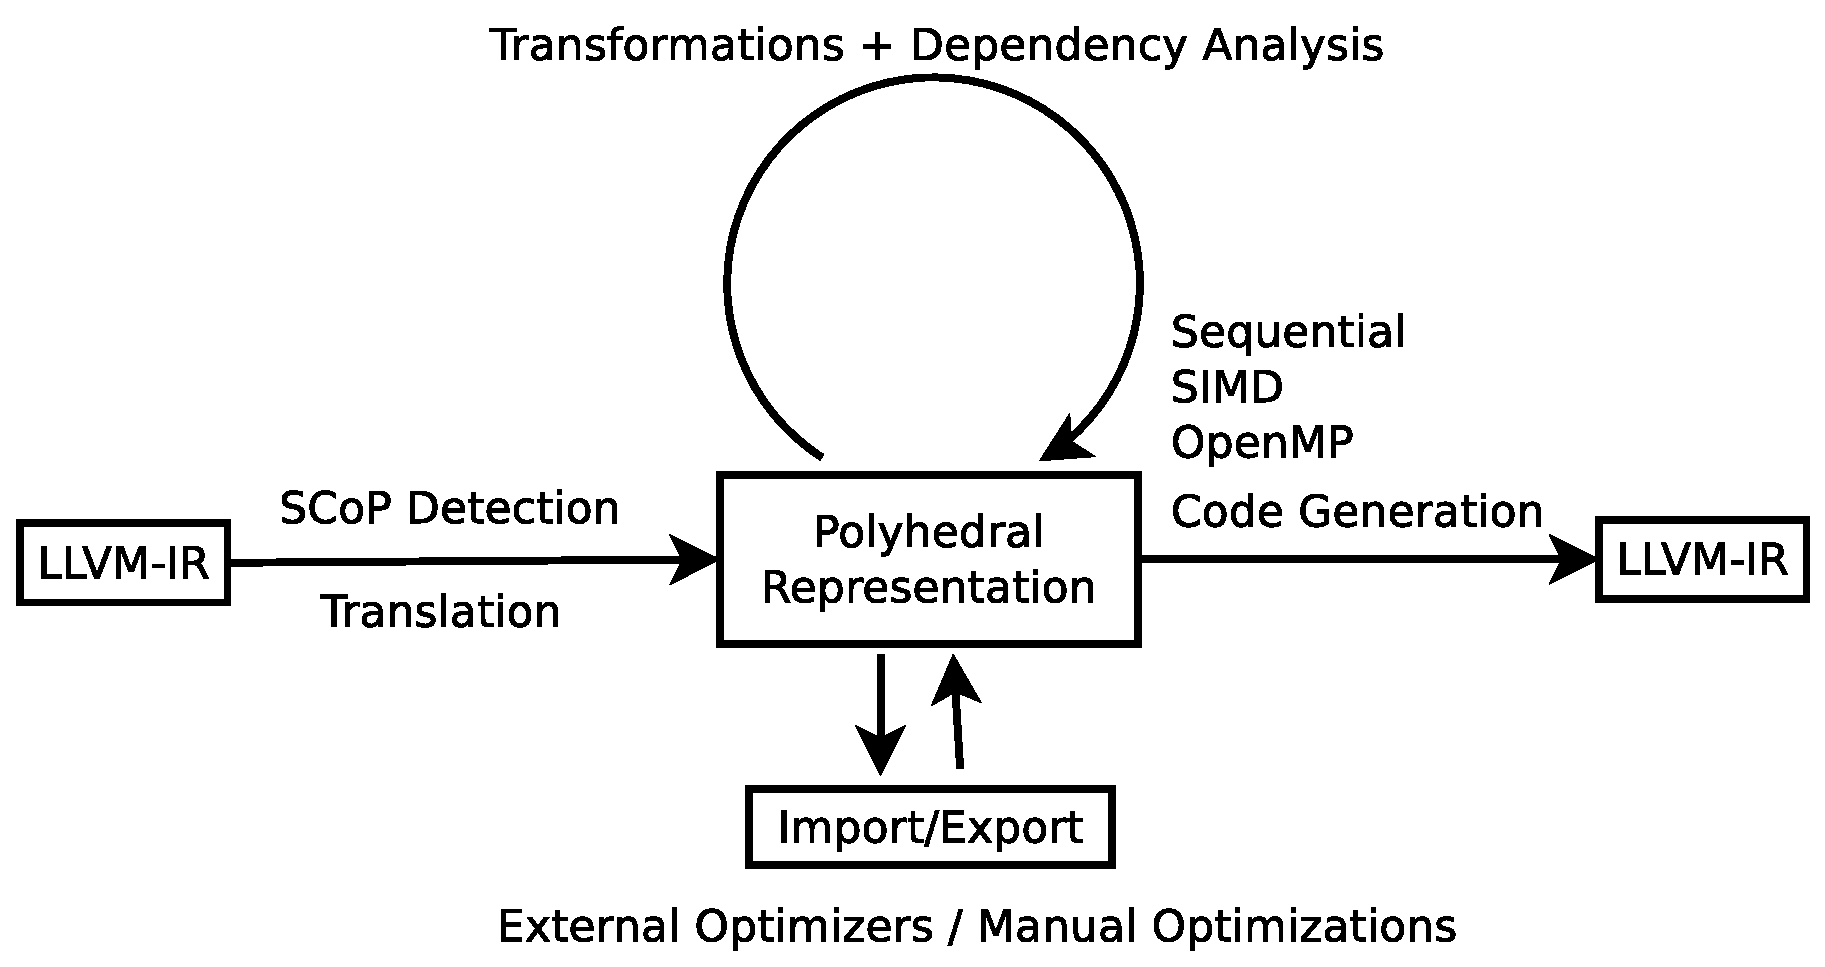
\includegraphics[width=1\textwidth]{images/architecture.eps}
  \caption{Architecture of Polly}
\end{figure}



%%%%%%%%%%%%%%%%%%%%%%%%%%%%%%%%%%%%%%%%%%%%%%%%%%%%%%%%%%%%
% openmp
\chapter{OpenMP Code Generation in Polly}
\label{chap:openmp}

\section{Introduction}
Transformations in Polly create loops that are executed in parallel, as if the user would have
added some OpenMP pragmas. To achieve this, code generation needs to emit code that calls OpenMP
library functions to be executed in parallel. The GNU OpenMP Library(libgomp) is used for this purpose. The
dependency analysis module of Polly automatically detects parallel loops(SCoPs) and are given to OpenMP
code generation module. Here we generate the required libgomp library calls. The generated code is similar
to the one generated if the user have added OpenMP pragmas\cite{parfor}. The following sections explain the steps
taken towards generating the OpenMP code. The generated code is in LLVM IR format.

\section{Generating OpenMP Library Calls}

Typically when a user want to run a particular section of the code in parallel he/she annotate the code with
OpenMP pragmas. The compiler will then convert this pragmas into the corresponding library calls. In Polly the
approach taken is to generate these calls automatically when a loop is detected as parallel.

Consider the for loop in ~\ref{fig:openmp1} to have a basic understanding about what is to be done.
This is detected as a parallel and given for OpenMP code generation. Here the following
sequence of GOMP library calls with proper arguments and return types(signature) has to be generated in
LLVM IR format.

\begin{figure}
\begin{lstlisting}
  for (int i = 0; i <= N; i++)
    A[i] = 1 ;
\end{lstlisting}
	\caption{An example}
	\label{fig:openmp1}
\end{figure}

\begin{itemize}
\item GOMP\_parallel\_loop\_runtime\_start
\item subfunction
\item GOMP\_parallel\_end
\end{itemize}

\begin{figure}
  \label{fig:openmp_cfg}
  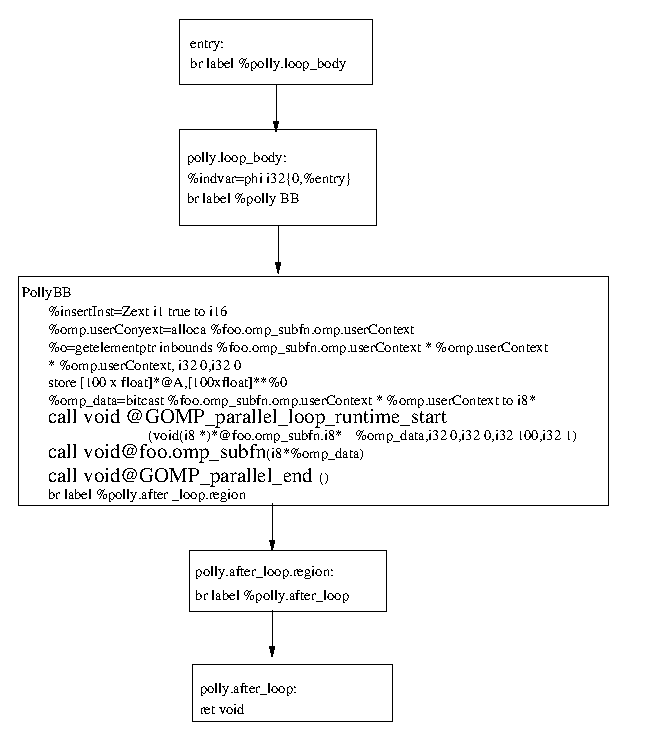
\includegraphics[width=1\textwidth]{images/ompcalls.eps}
  \caption{CFG showing sequence of OpenMP library calls}
\end{figure}

The control flow graph corresponding to the simple code in ~\ref{fig:openmp1} is shown in ~\ref{fig:openmp_cfg}
The code for body of the for loop is generated inside the subfunction which has the following GOMP library
calls to achieve the necessary parallelism.

\begin{itemize}
\item GOMP\_loop\_runtime\_next
\item GOMP\_loop\_end\_nowait
\end{itemize}

The signature and descriptions of each of the above functions can be found in in libgomp manual\cite{libgomp}.

\section{Support for inner loops}

So far OpenMP code created apply only for outermost loops, which is detected as SCoP. Next step is to do it for
inner loops. Due to dependency issues the outer loop is not detected as SCoP, but innerloop can be safely
parallelized as in the following example.

\begin{lstlisting}
  for (int i = 0; i < M; i++)
    for (int j = 0; j < N; j++)
      A[j] += M;
\end{lstlisting}

Those loops need the values of the surrounding induction variables and parameters in the OpenMP subfunction. We need
to pass the values of the outer induction variables in a structure to the subfunction. All the required variables
were already available in a data structure used by Polly. We just needed to copy those into the body of the subfunction
so that it can refer those whenever needed.

\section{Adding OpenMP testcases}

<give more explanation>

\section{Dealing with memory references}

\begin{lstlisting}
#define N 10
  void foo() {
    float A[N];
    for (int i=0; i < N; i++)
      A[i] = 10;
    return;
}
\end{lstlisting}

Consider the above code segment. The 'for' loop will be detected as parallel by Polly and will be embedded in the
body of the OpenMP subfunction. But it accesses a non-global array 'A' and so accessing the same will not be possible inside
the subfunction. The approach for solving this issue is explained below.

\subsection{Adding memory references}

The base addresses of all memory references made by a statement is available in each statement instance. Prior to creating the body
of the subfunction we add all these base addresses are added into the same data structure where we stored the induction variables and parameters.
And then it is added to the subfunction structure.

\subsection{Extracting memory references}

Inside the body of the subfunction the base addresses are extracted from the subfunction structure and a new LLVM load instruction is created for each. The
new base addresses mapped to the old addresses so that any future references are made on the new addresses.



%%%%%%%%%%%%%%%%%%%%%%%%%%%%%%%%%%%%%%%%%%%%%%%%%%%%%%%%%%%%
% testing
\chapter{Testing With Polybench}
\label{chap:testing}
\section{Polybench}

\section{Results}

\begin{figure}
\begin{center}
  \label{fig:2core1}
  %\includegraphics[width=1\textwidth]{images/2core32bit.eps}
  \includegraphics[height=9cm]{images/2core32bit.eps}
  \caption{Performance comparison}
\end{center}
\end{figure}

\begin{figure}
\begin{center}
  \label{fig:2core2}
  %\includegraphics[width=1\textwidth]{images/2core64bit.eps}
  \includegraphics[height=10cm]{images/2core64bit.eps}
  \caption{Performance comparison}
\end{center}
\end{figure}

\begin{figure}
\begin{center}
  \label{fig:10core}
  %\includegraphics[width=1\textwidth]{images/10core64bit.eps}
  \includegraphics[height=10cm]{images/2core64bit.eps}
  \caption{Performance comparison}
\end{center}
\end{figure}

%%%%%%%%%%%%%%%%%%%%%%%%%%%%%%%%%%%%%%%%%%%%%%%%%%%%%%%%%%%%
% testing
\chapter{Future Work and Conclusion}
\label{chap:future}
\section{Support for memory access transformations in Polly}
An improvement that can be made to polly is to add support for memory access transformations in Polly.
In many cases it would be great to change the pattern of memory access to obtain better data locality.
This can remove dependences that would otherwise block transformations and it can allow LLVM to use registers to store such values.

Polly performs its optimization on LLVM-IR based on the polyhedral model. Currently the transformations can be applied on Schedule (Order of computations)
Transformations can also be applied on the Memory Access (Pattern of memory access). A proper memory access transformation can improve data locality. This will in turn improve parallelism.

\section{Increasing Coverage of Polly}

Polly (Polyhedral optimization framework in LLVM) is showing very nice results for
several testcases. Yet, lot of larger test cases needs to be improved. we can explore
the reasons for this, find solutions for those and implement it. There are two parts for this.

\subsection{Increasing SCoP coverage}

The number of SCoPs detected need to be improved. This can be called as "Increasing SCoP Coverage". 

Expressions like min, max, sext, zext, trunc or unsigned comparisons in the loop bounds or memory
accesses are not handled in the current implementation. For example consider the following loop.
{\footnotesize
\begin{lstlisting}
for (int i = 0; i < N; i++)
  A[i] = B[i] + C[i];
\end{lstlisting}
}
In this case a sext is necessary if the code is translated to LLVM-IR and keep i as an i32 and
use an i64 to calculate the access to A[i]. This is  not currently handled in Polly.

Overflows NSW(No signed wrap) or NUW(No unsigned wrap) are not handled in the current implementation. So
it is not safe to compile a large project with Polly.

\subsection{Increasing the System Coverage}

Some of the testcases are failing when Polly is tested in machines which does not
have 64-bit Operating system. This needs to be fixed and can be called as "Increasing the System Coverage".
This can also be treated as porting to Polly to more architectures.
A solution for this issue could be to derive the data type needed by the maximal possible value a variable can have.

\section{Integrating Profile Guided Optimization into Polly}
An improvement that can be made to Polly is integrating profile guided optimization
\cite{pgo}. The idea is explained below with a few examples. Consider the following code.
{\footnotesize
\begin{lstlisting}
scanf("%d", &b);
for(i = 0; i < N; i +=  b) {
    body;
}
\end{lstlisting}
}
Polly will not detect this as a SCoP because the variable b is read as an user
input. So to detect this as a SCoP we instrument the IR with the information
provided by profiling. Suppose using profiling we figure out that most of the 
time the value of b is say 2. we can convert the above code as follows.
%\begin{verbatim}
{\footnotesize
\begin{lstlisting}
scanf("%d", &b);
if(b == 2) {
  for(i = 0; i < N; i += 2) {
      body;
  }
} else {
    for(i = 0; i < N; i += b) {
        body;
    }
}
\end{lstlisting}
}
Now with the transformed code the for loop inside 'if' will be detected as a 
SCoP and can be parallelised. Since value of N is 100 most of the time, the 
overall performance will be improved.

Consider another scenario.
{\footnotesize
\begin{lstlisting}
  for(i = 0; i < N; i++) {
      body;
  }
\end{lstlisting}
}
Suppose using profiling we know that N is always very small. So there wont be
much gain from parallelising it. So we have to tell polly that don't detect
this as a SCoP if N is less than a specific value.

Integrating such versioning we can expect to get heavily optimized performance 
for some often used cases.





%%%%%%%%%%%%%%%%%%%%%%%%%%%%%%%%%%%%%%%%%%%%%%%%%%%%%%%%%%%%
% gccvsllvm
%\chapter{Comparison of GCC and LLVM}
%\input{gcc_and_llvm.tex}

%%%%%%%%%%%%%%%%%%%%%%%%%%%%%%%%%%%%%%%%%%%%%%%%%%%%%%%%%%%%


% Appendices.

\appendix
 
\chapter{Various Tools Used in Polyhedral Community}
Some of the tools used in polyhedral community is described here with one example.
\section{ClooG}
CLooG is a free software and library generating loops for scanning Z-polyhedra.
It finds a code that reaches each integral point of one or more parameterized polyhedra.
CLooG has been written to solve the code generation problem for optimizing compilers based on the polytope model.

This is explained here with a simple example. Suppose we need to generate code for
a polyhedra with the following iteration domain.

\begin{center}
$D_{S}\ =\ \{(i,j)\ \epsilon\ Z^2\ |\ 2\ \leq\ i\ \leq\ 6\ \wedge\ 2\ \leq\ j\ \leq\ 6\ \wedge\ i\ \leq\ j\}$
\end{center}
We can give input to cloog as file which has the following format.
{\footnotesize
\begin{lstlisting}
# ---------------------- CONTEXT ------------------
c # language is C
# Context (constraints on two parameters)
2 4                   # 2 lines and 4 columns
# eq/in m  n  1   eq/in: 1 for >=0, 0 for =0
0   1  0 -6       # 1*m + 0*n -6*1 >= 0, i.e. m=6
0   0  1 -6       # 0*m + 1*n -6*1 >= 0, i.e. n=6
1 # We want to set manually the parameter names
m n                   # parameter names
# --------------------- STATEMENTS ----------------
1 # Number of statements
1 # First statement: one domain
# First domain
5 6                   # 5 lines and 6 columns
# eq/in i  j  m  n  1
1   1  0  0  0 -2 # i >= 2
1  -1  0  0  1  0 # i <= n
1   0  1  0  0 -2 # j >= 2
1   0 -1  1  0  0 # j <= m
1  -1  1  0  0  0 # n+2-i>=j
0  0  0               # for future options
1 # We want to set manually the iterator names
i j                   # iterator names
# --------------------- SCATTERING ---------------
0 # No scattering functions
\end{lstlisting}
}
Giving this file to 'cloog' command  as input it will generate the following code.
{\footnotesize
\begin{lstlisting}
/* Generated from ex1.cloog by CLooG 0.16.2 gmp bits in 0.00s. */
for (i=2;i<=6;i++) {
  for (j=i;j<=6;j++) {
    S1(i,j);
  }
}
\end{lstlisting}
}

\section{PLUTO}
PLUTO is an automatic parallelization tool based on the polyhedral model. The polyhedral model
for compiler optimization is a representation for programs that makes it convenient to perform
high-level transformations such as loop nest optimizations and loop parallelization. Pluto transforms
C programs from source to source for coarse-grained parallelism and data locality simultaneously.
The core transformation framework mainly works by finding affine transformations for efficient
tiling and fusion, but not limited to those.
Suppose we want to generate the tiled version of lu.c just issue the command
./polycc --tile lu.c
which will generate the output in a separate file called lu.tiled.c and displays
the following information
{\footnotesize
\begin{lstlisting}
[Pluto] Number of statements: 2
[Pluto] Total number of loops: 5
[Pluto] Number of deps: 10
[Pluto] Maximum domain dimensionality: 3
[Pluto] Number of parameters: 1
[Pluto] Affine transformations [<iter coeff's> <const>]
T(S1): (k, j, k)
3 3
 1  0  0 
 0  1  0 
 1  0  0 
T(S2): (k, j, i)
3 4
 1  0  0  0 
 0  0  1  0 
 0  1  0  0 
t1 --> fwd_dep  loop   (band 0)
t2 --> fwd_dep  loop   (band 0)
t3 --> fwd_dep  loop   (band 0)
[Pluto] Outermost tilable band: t0--t2
[Pluto] After tiling:
t1 --> fwd_dep  tLoop  (band 0)
t2 --> fwd_dep  tLoop  (band 0)
t3 --> fwd_dep  tLoop  (band 0)
t4 --> fwd_dep  loop   (band 0)
t5 --> fwd_dep  loop   (band 0)
t6 --> fwd_dep  loop   (band 0)
[Pluto] using Cloog -f/-l options: 4 6
[Polycc] Output written to ./lu.tiled.c
\end{lstlisting}
}
\section{VisualPolylib}
This is a tool using which we can visualize various operations on polyhedra. The polyhedral
description is given in a file and given as input to the 'visualpolylib' command.
For instance consider the following input
\begin{figure}
\begin{center}
  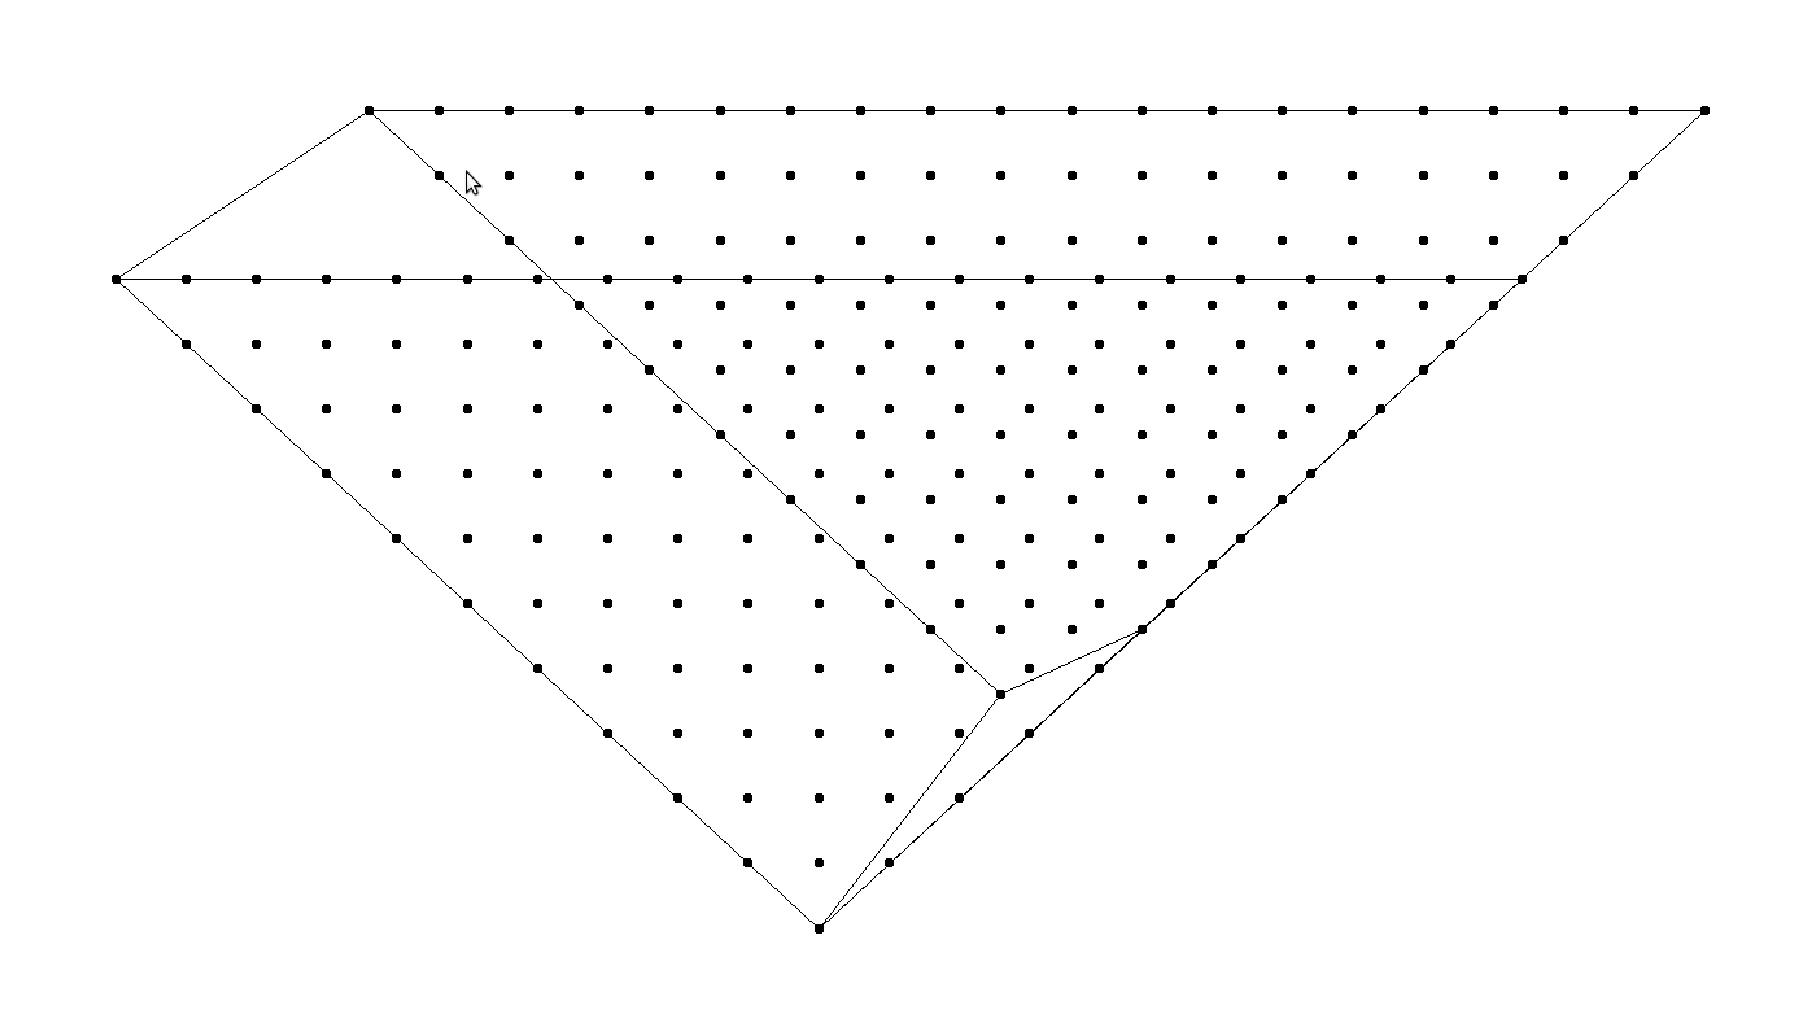
\includegraphics[width=1\textwidth]{images/3d.eps}
  \caption{Visualizing polyhedra with VisualPolylib}
  \label{fig:3d}
\end{center}  
\end{figure}

{\footnotesize
\begin{lstlisting}
P :=   { i, j, k | k <= 1, k >= 0, i <= j, i+j >= k, i+4k <= 4j,j<=10};
C:={|};
CS := { i,j,k | i-2j+2k<=0};
P2 := CS . P;
initvisu(3,C)
\end{lstlisting}
}
The polyhedra for P2 which is the intersection of CS and P can be viewed graphically as in 
Figure ~\ref{fig:3d}

\chapter{Doing Projects - The Open Source Way}
 
%%%%%%%%%%%%%%%%%%%%%%%%%%%%%%%%%%%%%%%%%%%%%%%%%%%%%%%%%%%%
% List of papers

\chapter*{Publications}
\vspace{-0.3cm}

\begin{enumerate}
\item Tobias Grosser, Hongbin Zheng, Raghesh Aloor, Andreas Simb{\"u}rger, Armin {G}r{\"o}{\ss}linger and Louis-No{\"e}l Pouchet \newblock
  Polly - Polyhedral optimization in LLVM \newblock {\em
  IMPACT 2011(First International workshop on PolyhedrAl Compilation Techniques)}, Chamonix, France.
\end{enumerate}

%\nocite{bellman, Amarel:1968, manning, knoblock90learning,
%crawford92theoretical, Barto:rtdp, Ravindran:proof}

%%%%%%%%%%%%%%%%%%%%%%%%%%%%%%%%%%%%%%%%%%%%%%%%%%%%%%%%%%%%
% Bibliography.
\pagebreak
\begin{singlespace}
  \begin{small}
	\bibliography{refs}
%\bibliographystyle{plain}
  \end{small}
\end{singlespace}

%%%%%%%%%%%%%%%%%%%%%%%%%%%%%%%%%%%%%%%%%%%%%%%%%%%%%%%%%%%%

\end{document}
